\section{Problem 5 - Random Forests}
\subsection{Finding Thresholds}
There are four places that I should take into consideration as possible thresholds.

\begin{center}
    \begin{tabular}{ |c|c|c| } 
     \hline
     option & $x_i$ & $x_{i+1}$ \\
     \hline
      1 & 20 & 30 \\ 
      2 & 60 & 70 \\
      3 & 90 & 100 \\
      4 & 100 & 110 \\ 
     \hline
    \end{tabular}
\end{center}
There hare four positions that could be possible threshold, however, I'm going to ignore
optinon 4, since it will be the same as option 1, except with reversed values.
These four places has been found using the same approatch as show in our
lecture, and lecture video (L10\_Classification\_Regression\_2\_Part3, starting at 17min 50sec.).
This means, that I'm only going to look at positions where there is a "change" in labels for 
a given datapoint compared to its predecessor or successor. Since there is no reason to look at possible thresholds where the neigbors to a given feature
has the same labels. 

This process can be formalized:
$$ x_i + (\frac{x_{i+1} - x_i}{2}): y_{i+1} \neq y_i $$

As stated, option 4 is the same as option 1, so I will only perform the calculations for option 1-3.

$$ \text{Option 1} = 20 + \frac{(30 - 20)}{2} = 25$$

$$ \text{Option 2} = 60 + \frac{(70 - 60)}{2} = 65$$

$$ \text{Option 3} =90 + \frac{(100 - 90)}{2} = 95$$
\\
Using my calculated values for for possible thresholds I have three different decision 
trees to take into consideration.
\\
\\
Tree 1:
\begin{figure}[H]
    \begin{center}
        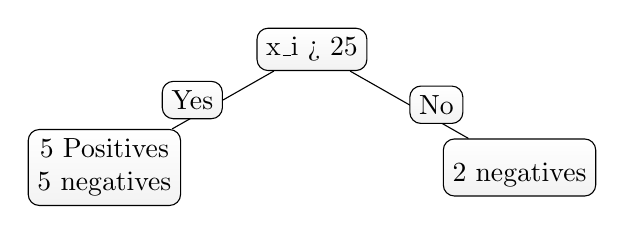
\begin{tikzpicture}
            [
                sibling distance  = 15em,
                every node/.style = {shape=rectangle, rounded corners,
                draw, align=center,
                top color=white, bottom color=lightgray!20}
            ]
            \node {x\_i > 25}
            child { node {5 Positives \\ 5 negatives} 
                edge from parent node [left] {Yes} }
            child { node {\\ 2 negatives} 
                edge from parent node [right] {No}};
        \end{tikzpicture}
    \end{center}
    \caption{Decision three with threshold = 25} \label{fig:M1}
\end{figure}
Tree 2:

\begin{figure}[H]
    \begin{center}
        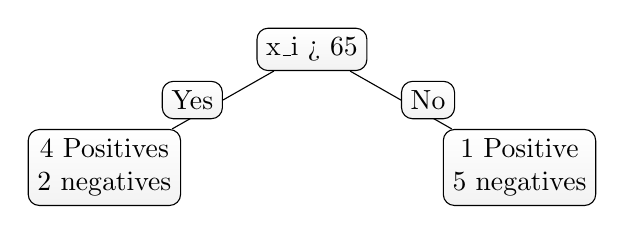
\begin{tikzpicture}
            [
                sibling distance  = 15em,
                every node/.style = {shape=rectangle, rounded corners,
                draw, align=center,
                top color=white, bottom color=lightgray!20}
            ]
            \node {x\_i > 65}
            child { node {4 Positives \\ 2 negatives} 
                edge from parent node [left] {Yes} }
            child { node {1 Positive \\ 5 negatives} 
                edge from parent node [right] {No}};
        \end{tikzpicture}
    \end{center}

    \caption{Decision three with threshold = 65} \label{fig:M2}
\end{figure}


Tree 3:

\begin{figure}[H]
    \begin{center}
        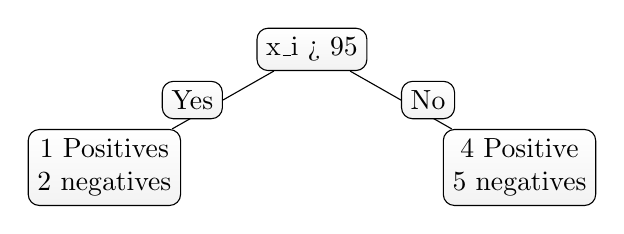
\begin{tikzpicture}
            [
                sibling distance  = 15em,
                every node/.style = {shape=rectangle, rounded corners,
                draw, align=center,
                top color=white, bottom color=lightgray!20}
            ]
            \node {x\_i > 95}
            child { node {1 Positives \\ 2 negatives} 
                edge from parent node [left] {Yes} }
            child { node {4 Positive \\ 5 negatives} 
                edge from parent node [right] {No}};
        \end{tikzpicture}
    \end{center}

    \caption{Decision three with threshold = 95} \label{fig:M3}
\end{figure}

From here, I will start by calculating the Entropy values for splits in my trees. Aswell as the information gain
using the functions ginven in our lecture slides (L10\_Classification\_Regression\_2\_Part3, p. 8)

$$\text{Entropy H(T)} = -p_+ \cdot log_2 \cdot p_+ - p_- \cdot log_2 \cdot  p_- $$

$$ \text{Gain (T, j)} = \text{H(T)} - \sum_{i = 0, 1} \frac{|T_i|}{|T|} \text{H}(T_i)$$

Calculating the information gain for tree 1 where the threshold is = 25:
\begin{align*}
     \text{Gain(T, j)} & = \text{H(5 pos, 7 neg)} - \frac{10}{12}\text{H(5 pos, 5 neg)} - \frac{2}{12}\text{H(0 pos, 2 neg)}\\
     & = 0.979 - \frac{10}{12} 1 - \frac{2}{12} 0 \approx 0.145
\end{align*}

Calculating the information gain for tree 2 where the threshold is = 65:
\begin{align*}
     \text{Gain(T, j)} & = \text{H(5 pos, 7 neg)} - \frac{6}{12}\text{H(4 pos, 2 neg)} - \frac{6}{12}\text{H(1 pos, 5 neg)}\\
     & = 0.979 - \frac{10}{12} 0.918 - \frac{2}{12} 0.650 \approx 0.195
\end{align*}

Calculating the information gain for tree 3 where the threshold is = 95:
\begin{align*}
     \text{Gain(T, j)} & = \text{H(5 pos, 7 neg)} - \frac{6}{12}\text{H(4 pos, 2 neg)} - \frac{6}{12}\text{H(1 pos, 5 neg)}\\
     & = 0.979 - \frac{10}{12} 0.918 - \frac{2}{12} 0.991 \approx 0.0062
\end{align*}

Since the goal is to find the tree which gives us the highest information gain. I can see that
the second decision tree with a threshold of 65 is the best one.

Thus, the optimal threshold is 65.

\newpage